\documentclass{standalone}
\usepackage[utf8]{inputenc}
\usepackage{tikz}
\usepackage{color}
\usetikzlibrary{arrows,shapes,positioning,shadows,trees}

\tikzset{
  basic/.style  = {draw, text width=3cm, drop shadow, font=\sffamily, rectangle},
  root/.style   = {basic, rounded corners=2pt, thin, align=center,
                   fill=blue!60},
  level 2/.style = {basic, rounded corners=6pt, thin,align=center, fill=blue!40,
                   text width=15em},
  level 3/.style = {basic, thin, align=left, fill=blue!20, text width=11em}
}

\begin{document}

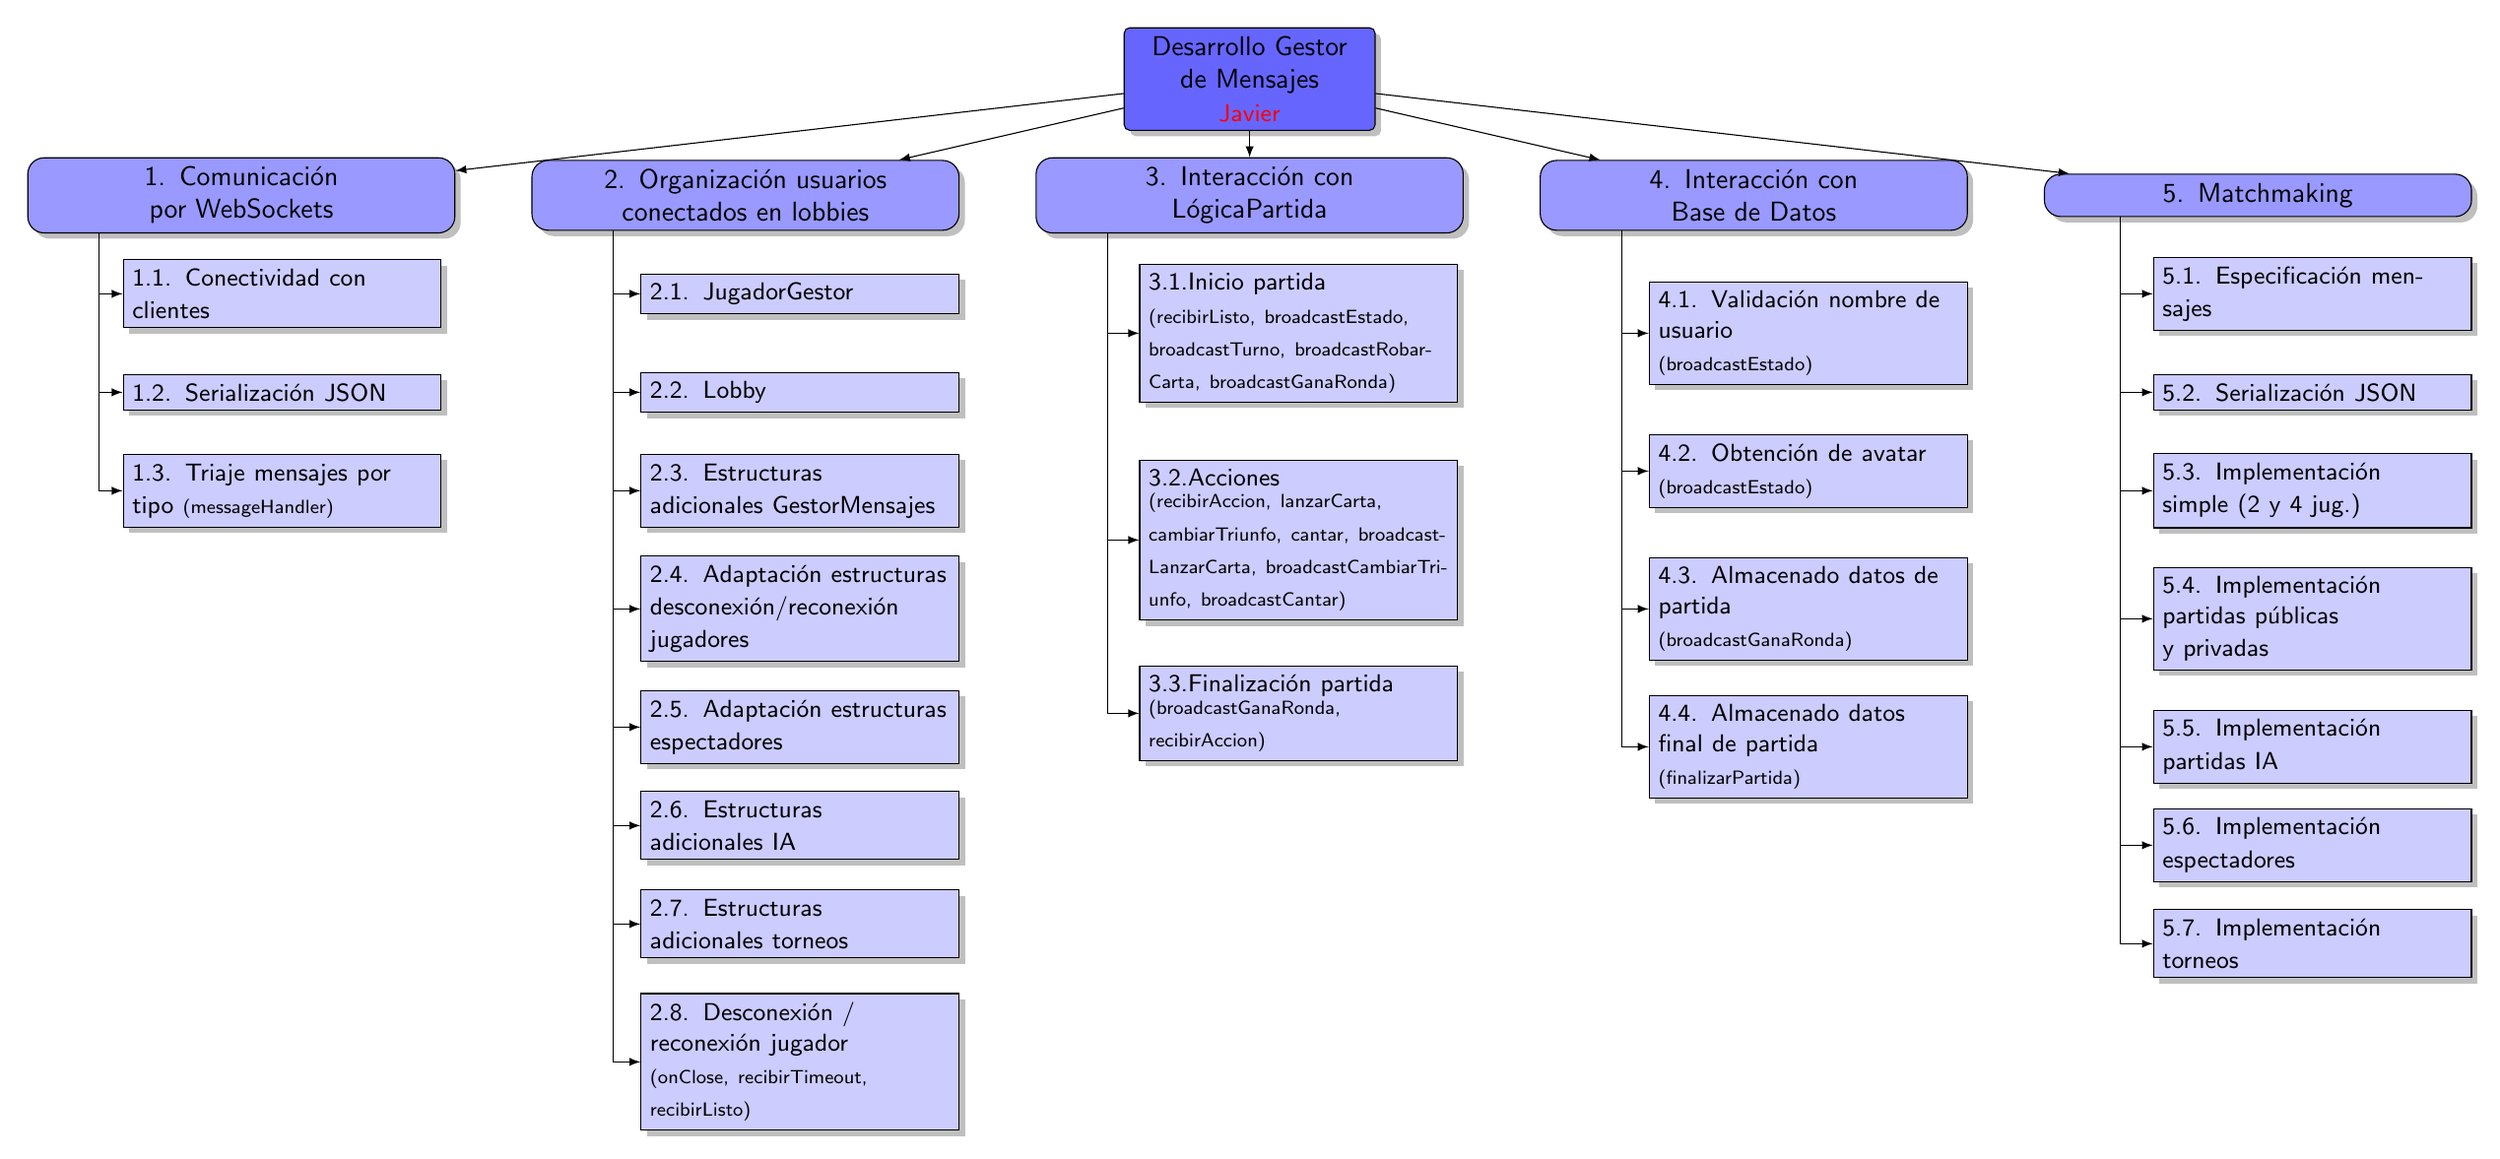
\begin{tikzpicture}[
  level 1/.style={sibling distance=65mm},
  edge from parent/.style={->,draw},
  >=latex]

% raiz inicial
\node[root] {Desarrollo Gestor de Mensajes \\ \textcolor{red}{\small{Javier}}}
% The first level, as children of the initial tree
  child {node[level 2] (c1) {1. Comunicación \\ por WebSockets}}
  child {node[level 2] (c2) {2. Organización usuarios \\ conectados en lobbies}}
  child {node[level 2] (c3) {3. Interacción con \\ LógicaPartida}}
  child {node[level 2] (c4) {4. Interacción con \\ Base de Datos}}
  child {node[level 2] (c5) {5. Matchmaking}};

% The second level, relatively positioned nodes
\begin{scope}[every node/.style={level 3}]
\node [below of = c1,node distance=0.5in, xshift=15pt] (c11) {\small{1.1. Conectividad con clientes}};
\node [below of = c11, node distance=0.5in] (c12) {\small{1.2. Serialización JSON}};
\node [below of = c12, node distance=0.5in] (c13) {\small{1.3. Triaje mensajes por tipo \scriptsize{(messageHandler)}}};

\node [below of = c2,node distance=0.5in, xshift=20pt] (c21) {\small{2.1. JugadorGestor}};
\node [below of = c21, node distance=0.5in] (c22) {\small{2.2. Lobby}};
\node [below of = c22, node distance=0.5in] (c23) {\small{2.3. Estructuras \\adicionales GestorMensajes}};
\node [below of = c23, node distance=0.6in] (c24) {\small{2.4. Adaptación estructuras \\ desconexión/reconexión jugadores}};
\node [below of = c24, node distance=0.6in] (c25) {\small{2.5. Adaptación estructuras \\ espectadores}};
\node [below of = c25, node distance=0.5in] (c26) {\small{2.6. Estructuras \\adicionales IA}};
\node [below of = c26, node distance=0.5in] (c27) {\small{2.7. Estructuras \\adicionales torneos}};
\node [below of = c27, node distance=0.7in] (c28) {\small{2.8. Desconexión / \\ reconexión jugador}\\ \scriptsize{(onClose, recibirTimeout, recibirListo)}};

\node [below of = c3, xshift=18pt, node distance = 0.7in] (c31) {\small{3.1.Inicio partida} \\ \scriptsize{(recibirListo, broadcastEstado, broadcastTurno, broadcastRobarCarta, broadcastGanaRonda)}};
\node [below of = c31, node distance = 1.05in] (c32) {\small{3.2.Acciones} \\ \scriptsize{(recibirAccion, lanzarCarta, \\cambiarTriunfo, cantar, broadcastLanzarCarta, broadcastCambiarTriunfo, broadcastCantar)}};
\node [below of = c32, node distance = 0.88in] (c33) {\small{3.3.Finalización partida} \\ \scriptsize{(broadcastGanaRonda, \\recibirAccion)}};

\node [below of = c4,xshift=20pt, node distance = 0.7in] (c41) {\small{4.1. Validación nombre de usuario} \\ \scriptsize{(broadcastEstado)}};
\node [below of = c41, node distance=0.7in] (c42) {\small{4.2. Obtención de avatar} \\ \scriptsize{(broadcastEstado)}};
\node [below of = c42, node distance=0.7in] (c43) {\small{4.3. Almacenado datos de partida} \\ \scriptsize{(broadcastGanaRonda)}};
\node [below of = c43, node distance=0.7in] (c44) {\small{4.4. Almacenado datos final de partida} \\ \scriptsize{(finalizarPartida)}};

\node [below of = c5,node distance=0.5in, xshift=20pt] (c51) {\small{5.1. Especificación mensajes}};
\node [below of = c51, node distance=0.5in] (c52) {\small{5.2. Serialización JSON}};
\node [below of = c52, node distance=0.5in] (c53) {\small{5.3. Implementación \\simple (2 y 4 jug.)}};
\node [below of = c53, node distance=0.65in] (c54) {\small{5.4. Implementación \\ partidas públicas \\ y privadas}};
\node [below of = c54, node distance=0.65in] (c55) {\small{5.5. Implementación \\ partidas IA}};
\node [below of = c55, node distance=0.5in] (c56) {\small{5.6. Implementación \\ espectadores}};
\node [below of = c56, node distance=0.5in] (c57) {\small{5.7. Implementación \\ torneos}};


\end{scope}


\foreach \value in {1,2,3}
  \draw[->] (c1.195) |- (c1\value.west);

\foreach \value in {1,...,8}
  \draw[->] (c2.195) |- (c2\value.west);

\foreach \value in {1,...,3}
  \draw[->] (c3.195) |- (c3\value.west);

\foreach \value in {1,...,4}
  \draw[->] (c4.195) |- (c4\value.west);

\foreach \value in {1,...,7}
  \draw[->] (c5.189) |- (c5\value.west);

\end{tikzpicture}

\end{document}
